%%%%%%%%%%%%%%%%%%%%%%%%%%%%%%%%%%%%%%
%%%%%%%%%%%%%%%%%%%%%%%%%%%%%%%%%%%%%%
% Do not edit the TeX file your work
% will be overwritten.  Edit the RnW
% file instead.
%%%%%%%%%%%%%%%%%%%%%%%%%%%%%%%%%%%%%%
%%%%%%%%%%%%%%%%%%%%%%%%%%%%%%%%%%%%%%





\newcommand{\DefineMacros}{
\newcommand{\NumRows}{3}

}


%%%%%%%%%%%%%%%%%%%%%%%

\newcommand{\ExamplePlot}{

\begin{knitrout}
\definecolor{shadecolor}{rgb}{0.969, 0.969, 0.969}\color{fgcolor}\begin{figure}[h!]

{\centering 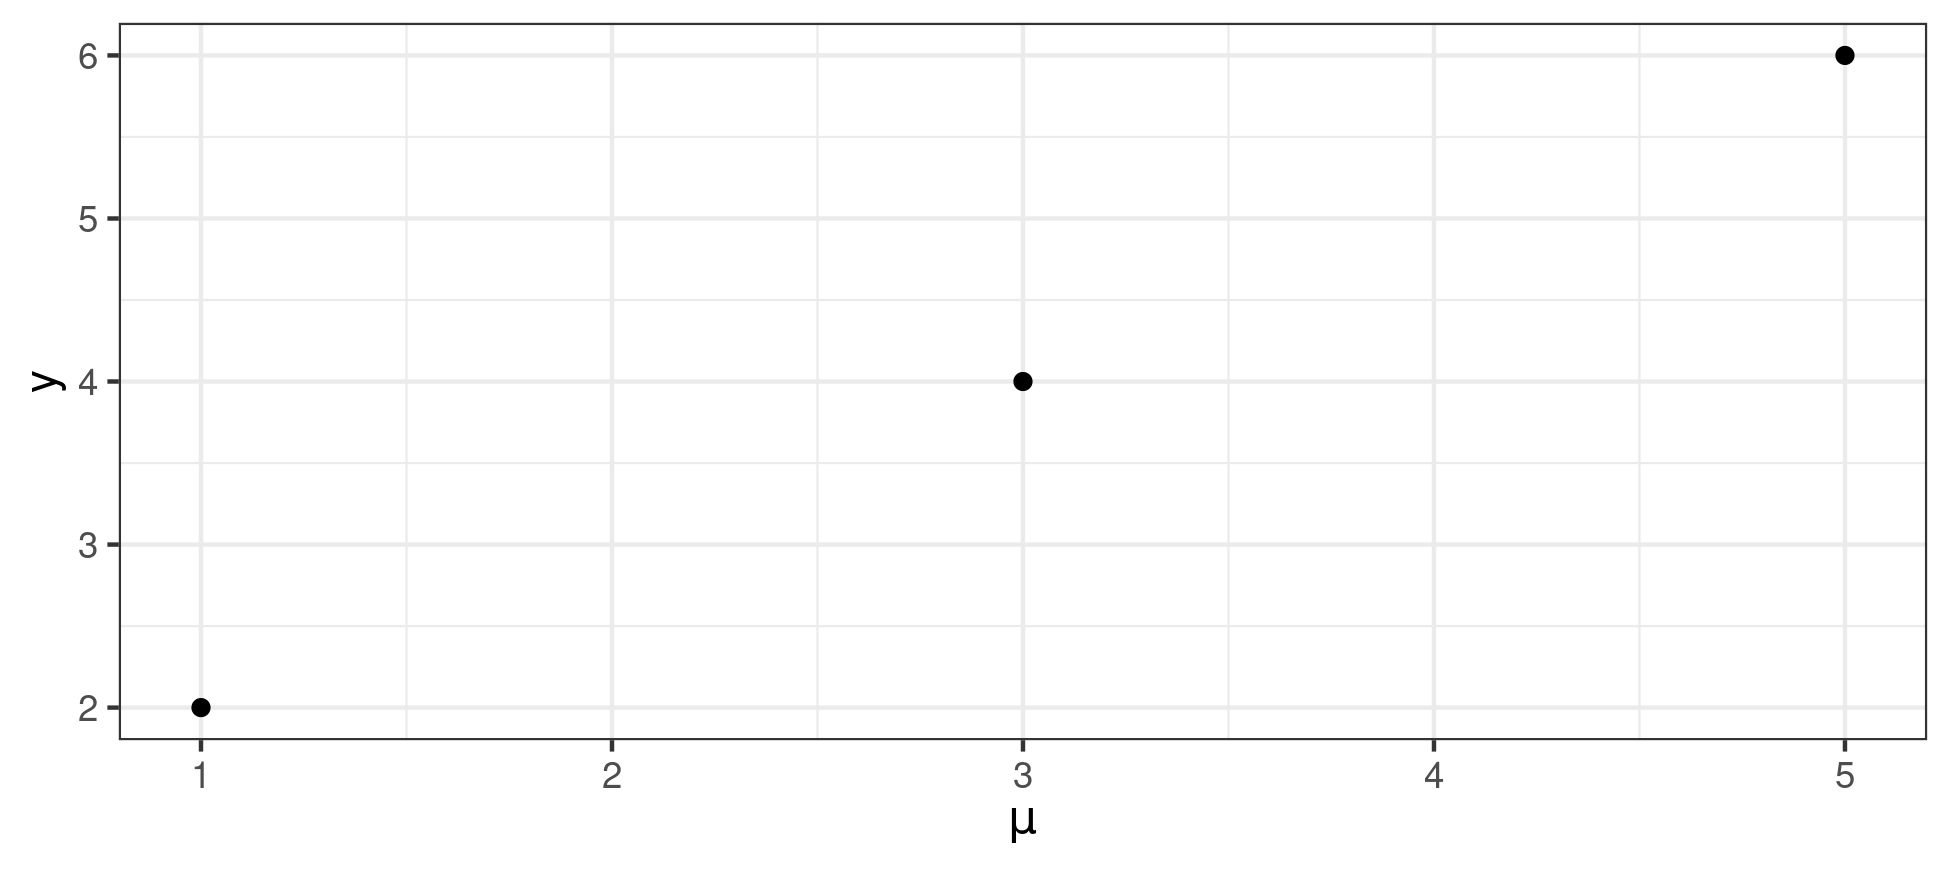
\includegraphics[width=0.98\linewidth,height=0.441\linewidth]{figure/exampleplot-1} 

}

\caption[]{Caption  here}\label{fig:exampleplot}
\end{figure}

\end{knitrout}
}



% %%%%%%%%%%%%%%%%%%%%%%

\newcommand{\ExampleTable}{

\begin{tabular}{r|r}
\hline
x & y\\
\hline
1 & 2\\
\hline
3 & 4\\
\hline
5 & 6\\
\hline
\end{tabular}

}
